\section{Auswertung}
%gaussian-A
%\begin{align*}
%	\sqrt{\frac{ln(2)}{\pi}} \cdot \frac{a}{dx} \cdot exp \left(-ln(2) \cdot \frac{(x-x0)^2}{dx^2} \right)
%\end{align*}
\subsection{Photolumineszenz-Eigenschaften der kolloidalen Nanokristalle}
Die erste Aufgabe ist es, einige Eigenschaften der kolloidalen Nanokristalle anhand von Photoluminezsenzspektren zu untersuchen.
\subsubsection{ Gr\"{o}{\ss}e der Nanokristalle}
Zun\"{a}chst soll die Gr\"{o}{\ss}e der kolloidalen Nanokristalle jeder Probe bestimmt werden.
Hierf\"{u}r wird jede Probe einzelne mit einem Laser der Wellenl\"{a}nge $405 \,$nm angeregt und ein Photoluminezsenzspektrum (PL-Spektrum) von ca $320$ - $747 \,$nm wird aufgenommen.
Diese PL-Spektren sind in Abbildung (\ref{abb:auf1a}) zu sehen. 
\begin{figure}[H]
\centering
	\begin{subfigure}[t]{0.4\textwidth}
	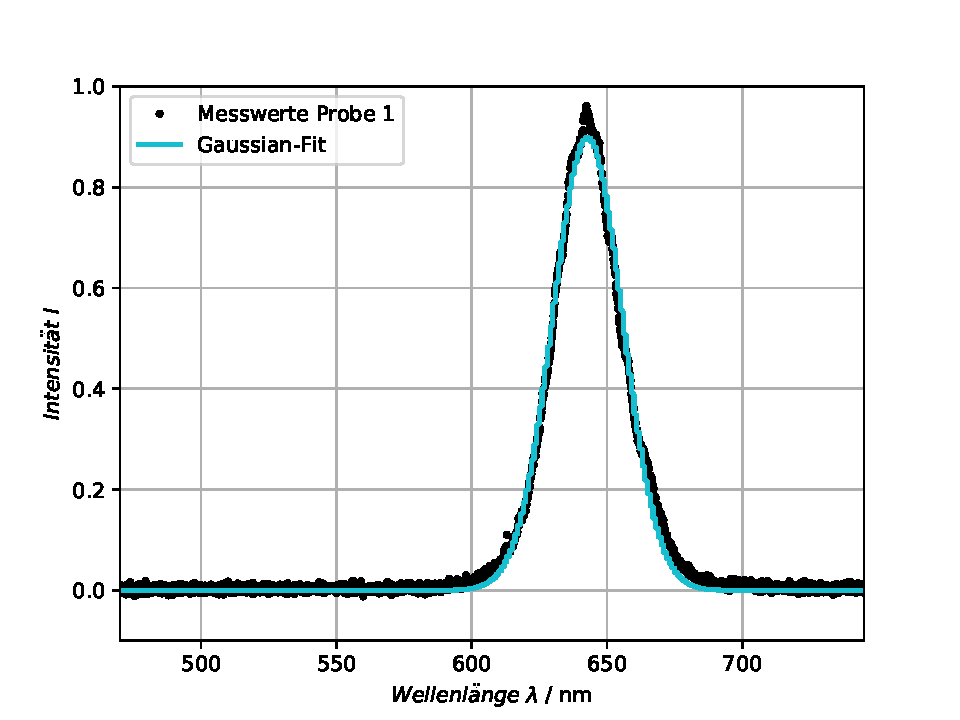
\includegraphics[width=\textwidth]{Plots/aufgabe1a_P1.pdf}
	\caption{Messung der Probe 1 mit Messdauer $1 \,$s.}
	\label{abb:A1_P1}
	\end{subfigure}
	~
	\begin{subfigure}[t]{0.4\textwidth}
	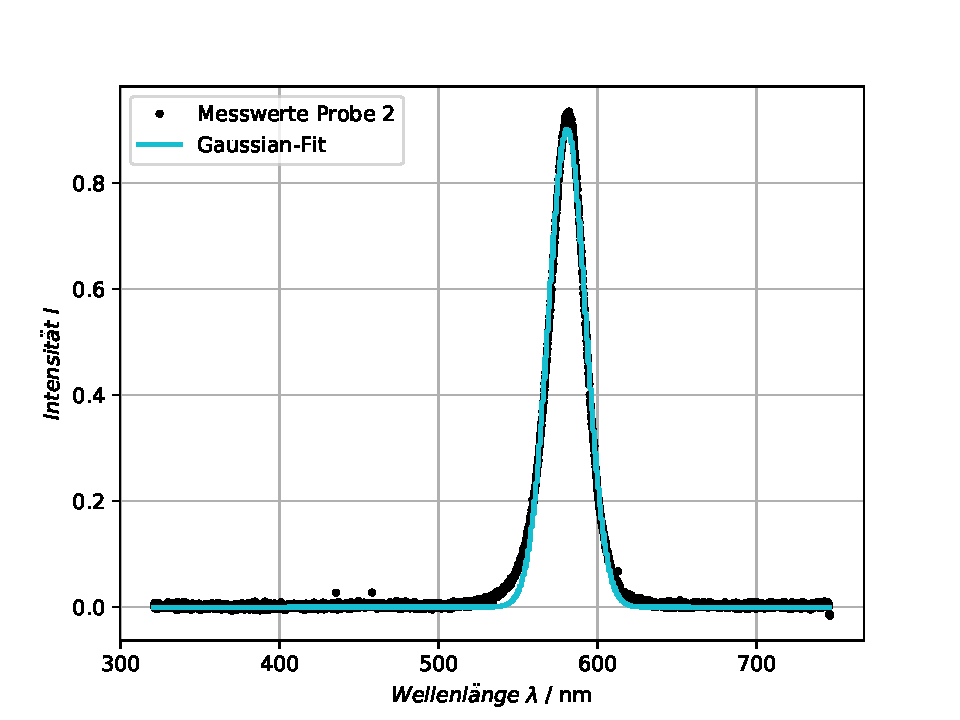
\includegraphics[width=\textwidth]{Plots/aufgabe1a_P2.pdf}
	\caption{Messung der Probe 2 mit Messdauer $0,5 \,$s.}
	\label{abb:A1_P2}
	\end{subfigure}
	~
	\begin{subfigure}[t]{0.4\textwidth}
	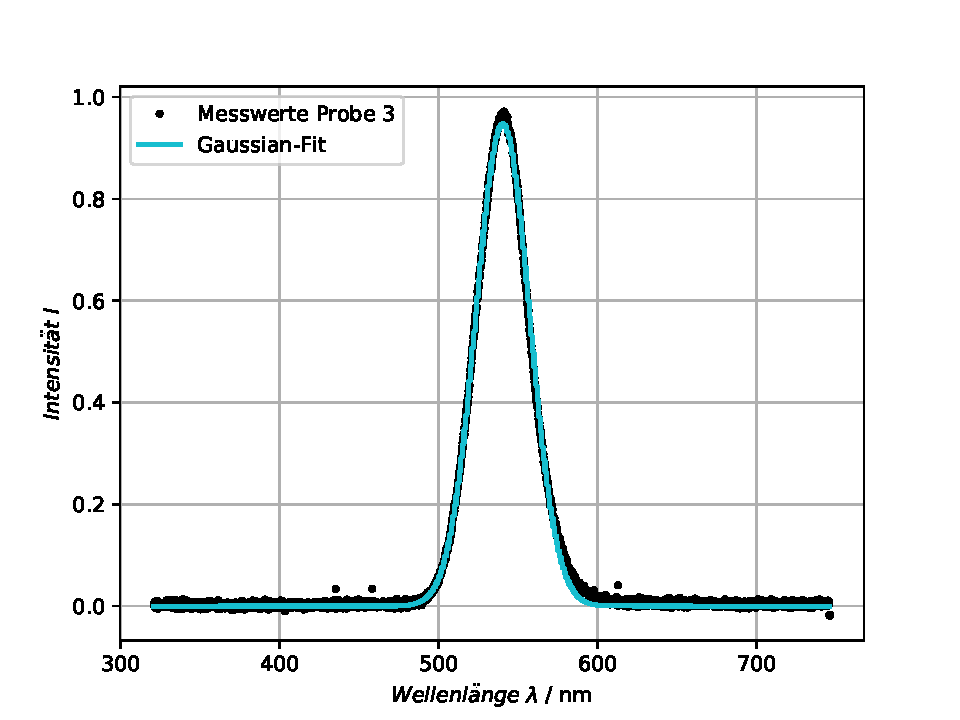
\includegraphics[width=\textwidth]{Plots/aufgabe1a_P3.pdf}
	\caption{Messung der Probe 3 mit Messdauer $0,65 \,$s.}
	\label{abb:A1_P3}
	\end{subfigure}
\caption{Photoluminessenzspektren der drei vorliegenden Proben mit einer Anregungswellenl\"{a}nge von 405 nm.}
\label{abb:auf1a}
\end{figure}
Alle drei Spektren weisen nur geringf\"{u}gige Abweichungen auf.
Mit Hilfe von Magicplots und Python werden durch die Messwerte aller drei Pl-Spektren gau{\ss}f\"{o}rmige Ausgleichskurven gelegt.
Diese besitzen die in Formel (\ref{form:gauss}) beschriebene Form.
\begin{align}
	y = a \cdot exp \left( -ln(2) \cdot \frac{(x-x_0)^2}{dx^2} \right)
\label{form:gauss}
\end{align}
Hierbei gibt $a$ die Amplitude und $dx$ die Linienbreite das Gau{\ss}kurve an.
Die Variable $x_0$ gibt die Wellenl\"{a}nge $\lambda_i$ der Probe an.
Mittels der Formeln (\ref{form:energie}) und (\ref{form:radius}) lassen sich nun die Gr\"{o}{\ss}e der Nanopartikel berechnen.
\begin{align}
	\Delta E_{r,i} &= h \frac{c}{\lambda_i} \label{form:energie}\\
	\Delta E_{r,i} &= E_g + \frac{h^2}{8r_{NP,i}} \left( \frac{1}{m_e^*} + \frac{1}{m_h^*} \right) \label{form:radius}
\end{align}
Alle Ergebnisse sind in Tabelle (\ref{tab:auf1a}) aufgelistet.
\begin{table}
	\centering
	\caption{Ergebnisse aus den Fit-Kurven der drei Messungen.}
\begin{tabular}{|r|cccc|}
	\hline
	{Probe} & \multicolumn{2}{c}{Wellenl\"{a}nge $\lambda_i$ / nm} & {Energie $E_{r,i}$ / eV} & {Radius $r_{NP}$ / nm} \\
	 & Theorie & experimentell &  &  \\
	\hline
	1	&	644	& 642,819 &	1,9289	&	7,717	\\
	2	&	580	& 580,832 &	2,1348	&	5,338	\\
	3	&	542	& 540,287 &	2,2949	&	4,502	\\
	\hline
\end{tabular}
\label{tab:auf1a}
\end{table}

\subsubsection{Polarisation der Photolumineszenz}
Im n\"{a}chsten Schritt wird an einer Probe beispielhaft untersucht, ob die Photoluminezsenz polarisiert ist.
In Abbildung (\ref{abb:polarisation}) sind die drei verschiedenen PL-Spektren der Probe drei zu sehen.
\begin{figure}[hbtp]
	\centering
	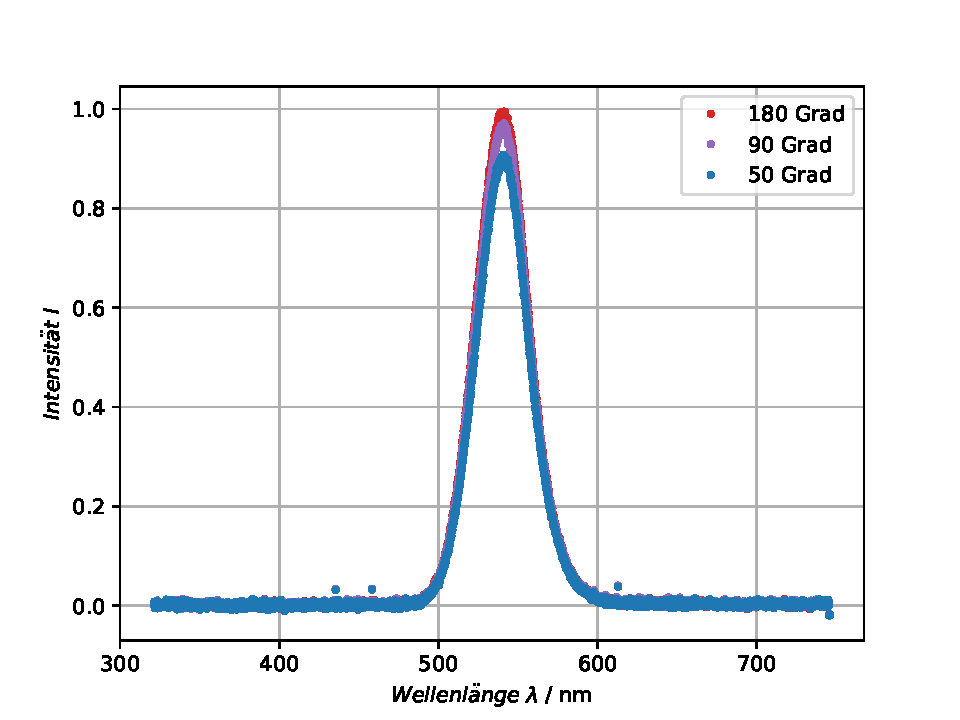
\includegraphics[width=0.5\textwidth]{Plots/aufgabe1b.pdf}
	\caption{PL-Spektren der Probe 3 mit einer Anregungswellenl\"{a}nge von $405 \,$nm f\"{u}r drei unterschiedliche Polarisationswinkel im Detektionspfad.}
	\label{abb:polarisation}
\end{figure}
Hier ist zu erkennen, dass f\"{u}r verschiedene Polarisationswinkel in der Detektion das Spektrum der Photoluminezsenz die selbe Form aufweist.
Lediglich die Intensit\"{a}t des Peaks variiert ein wenig.
%Je gr\"{o}{\ss}er der Polarisationswinkel desto h\"{o}her ist die Intensit\"{a}t der Photoluminezsenz.
Doch die Photoluminezsenz der Nanokristalle ist unpolarisiert.

\subsubsection{Leistungsabh\"{a}ngige Peak-Energie}
Als letzte Eigenschaft wird die Peak-Energie in Abh\"{a}ngigkeit der Leistung untersucht.
Auch diese Messung wird wieder an der Probe 3 durchgef\"{u}hrt.
F\"{u}r sieben verschiedenen Laserleistungen wird das PL-Spektrum aufgenommen.
Um keine S\"{a}ttigung des Detektors zu erreichen, wird die Messzeit f\"{u}r jede Laserleistung variiert.
In Tabelle (\ref{tab:1c}) sind die Messwerte zu den Spektren notiert.
\begin{table}
	\centering
	\caption{Aufgenommene Werte der Messungen zur Leistungsabh\"{a}ngige Peak-Energie.}
%\begin{tabular}{|D{.}{,}{-1}cc|}
\begin{tabular}{|ccc|}
	\hline
	{Laserleistung / mW} & {Intensi\"{a}t} & {Zeitintervall $\Delta t$ / ms} \\
	\hline
	0,1	&	0,3311	&	1800	\\
	0,5	&	0,8477	&	1200	\\
	1	&	0,9658	&	700	\\
	5	&	0,9684	&	150	\\
	10	&	0,9286	&	70	\\
	15	&	0,9687	&	50	\\
	20	&	0,7922	&	30	\\
	\hline
\end{tabular}
\label{tab:1c}
\end{table}
Die aufgenommenen PL-Spektren werden mit Formel (\ref{form:gauss}) gefittet.
Um sie untereinander besser vergleichen zu k\"{o}nnen werden die PL-Spektren f\"{u}r eine Messzeit von $1 \, s$ umgerechnet.
In Abbildung (\ref{abb:verLeistung2}) sind diese Kurven zu sehen.
\begin{figure}[H]
\centering
%	\begin{subfigure}[t]{0.45\textwidth}
%	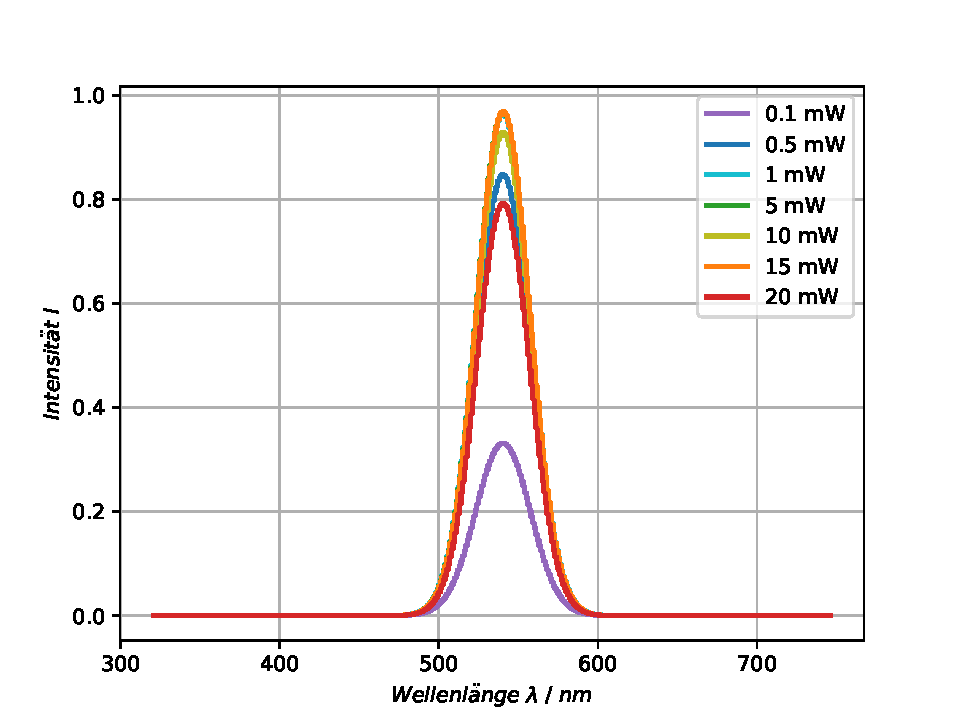
\includegraphics[width=\textwidth]{Plots/aufgabe1c2.pdf}
%	\caption{Die aufgenommenen PL-Spektren f\"{u}r verschiedenen Laserleistungen.}
%	\label{abb:verLeistung}
%	\end{subfigure}
%	~
	\begin{subfigure}[t]{0.45\textwidth}
	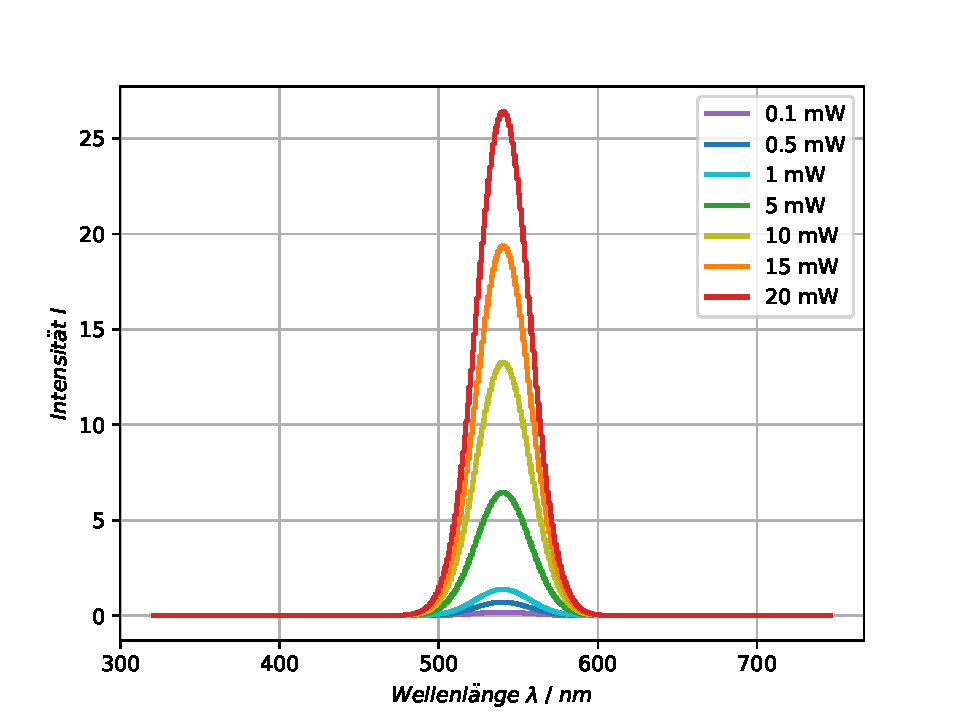
\includegraphics[width=\textwidth]{Plots/aufgabe1c2_1s.pdf}
	\caption{Die Fit-Kurven zu den aufgenommenen PL-Spektren f\"{u}r verschiedenen Laserleistungen mit einer Messzeit von $1$ s.}
	\label{abb:verLeistung2}
	\end{subfigure}
	~
	\begin{subfigure}[t]{0.45\textwidth}
	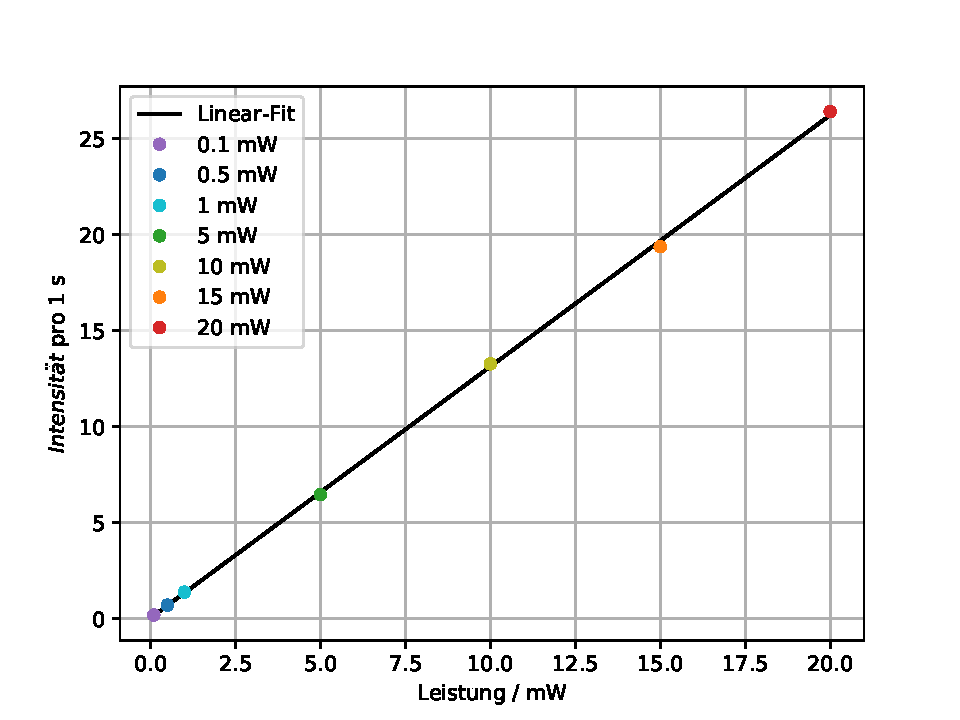
\includegraphics[width=\textwidth]{Plots/aufgabe1c3.pdf}
	\caption{Die Peak-Energien der PL-Spektren mit linearem Fit.}
	\label{abb:Leistungen_fit}
	\end{subfigure}
\caption{Messung der Peak-Energie der Probe 3 mit einer Anregungswellenl\"{a}nge von $405 \,$nm f\"{u}r unterschiedliche Laserleistungen.}
\label{abb:auf1c}
\end{figure}
Die Leistung der Peakmaxima sind in Abbildung (\ref{abb:Leistungen_fit}) gegen die Intensit\"{a}t aufgetragen.
Der lineare Fit bestizt die Form:
\begin{align*}
	I_{Peak} = (1,30995 \pm 0,00932) \cdot P_{Laser} + (0,02559 \pm 0,09654)
\end{align*}

Aus dem Fit lassen sich Linienbreite und Amplitude der Peaks ablesen.
Mittels Formel (\ref{form:energie}) lassen sich die Emissionsenergien der Paeks bestimmen.
Die Messergebnisse sind in Tabelle (\ref{tab:1c_2}) aufgelistet.
\begin{table}
	\centering
	\caption{Ergebnisse der Messung zur Leistungsabh\"{a}ngige Peak-Energie und ihrer Linienbreite f\"{u}r eine Messzeit von $1 \, s$.}
\begin{tabular}{|cccc|}
	\hline
	{Laserleistung / mW}	&	{Emissionsenergie / eV}	&	{Linienbreite / meV}	&	{Amplitude}	\\
	\hline
	0,1	&	2,2943037	&	20,2138	&	0,18394	\\
	0,5	&	2,2942871	&	19,9469	&	0,70642	\\
	1	&	2,2944082	&	19,8745	&	1,37971	\\
	5	&	2,2943158	&	19,7709	&	6,45600	\\
	10	&	2,2940935	&	19,7519	&	13,26570	\\
	15	&	2,2939390	&	19,7476	&	19,37400	\\
	20	&	2,2939810	&	19,6778	&	26,40667	\\
	\hline
	\end{tabular}
\label{tab:1c_2}
\end{table}
In Abbildung (\ref{abb:auf1c_ergebnisse}) sind Linienbreite und Emissionsenergie gegn die angelegte Laserleistung aufgetragen.
\begin{figure}[hbtp]
\centering
	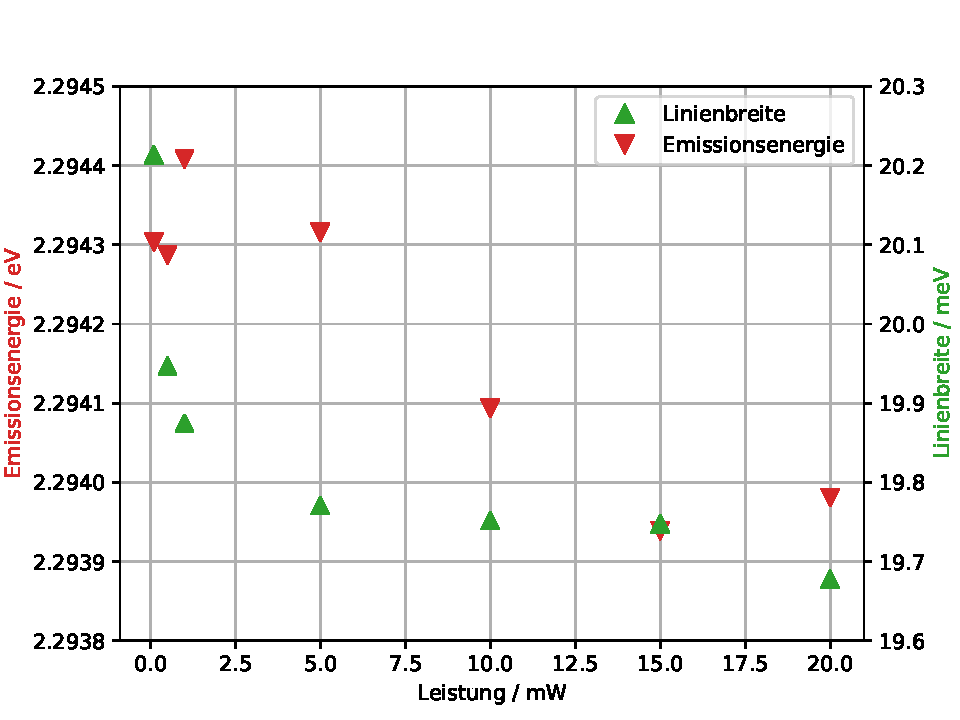
\includegraphics[width=0.6\textwidth]{Plots/aufgabe1c4.pdf}
	\caption{Die Emissionsenergie der Probe 3 mit Wellenl\"{a}nge $540,287 \,$nm in Abh\"{a}ngigkeit der Laserleistung.}
	\label{abb:auf1c_ergebnisse}
\end{figure}
Zu sehen ist, dass die Linienbreite mit steigender Laserleistung erste stark und dann immer flacher abf\"{a}llt.
Im Gegensatz dazu steigt die Emissionsenergie kurz an, bevor diese mit steigenden Laserleistung sinkt, um bei der letzten Messung wieder etwas zu steigen.

\subsection{Abhängigkeit der Photolumineszenz von der Laserwellenlänge}
In der zweiten Messreihe werden wieder alle drei Probe untersucht.
Diesmal werden die Proben mit unterschiedlichen Wellenl\"{a}ngen angeregt.
Verwendet werden Laser mit den Wellenl\"{a}nen $448 \,$nm, $518 \,$nm und $636 \,$nm.
Zum Vergleich sind in den folgenden PL-Spektren auch immer das PL-Spektrum der jeweiligen Probe aus dem ersten Aufgabenteil dargestellt, siehe Abbildung (\ref{abb:auf1a}).
In den Graphen (\ref{abb:auf2p1a}), (\ref{abb:auf2p2a}) und (\ref{abb:auf2p3a}) sind die Messwerte dargestellt.
Auch hier wurden, wie zuvor auch schon, die Messwerte f\"{u}r eine Messzeit von $1 \, s$ hochgerechnet, um die Sprktren besser miteinander vergleichen zu k\"{o}nnen.
Zu sehen sind dabei jeweils in jedem Spektrum ein sehr schmaler Peak und ein breitere.
Ersterer ist der Reflexions-Peak und stammt von dem Laser, mit dem die Probe angeregt wird.
Der breitere PL-Peak wird mit der Formel (\ref{form:gauss}) gefittet und ist jeweils in dem Graphen rechts daneben dargestellt.

In Abbildung (\ref{abb:auf2p1b}) ist zu sehen, dass die Nanokristalle der Probe 1 mit allen vier Wellenl\"{a}ngen angeregt werden k\"{o}nnen.
\begin{figure}[hbtp]
\centering
	\begin{subfigure}[t]{0.45\textwidth}
	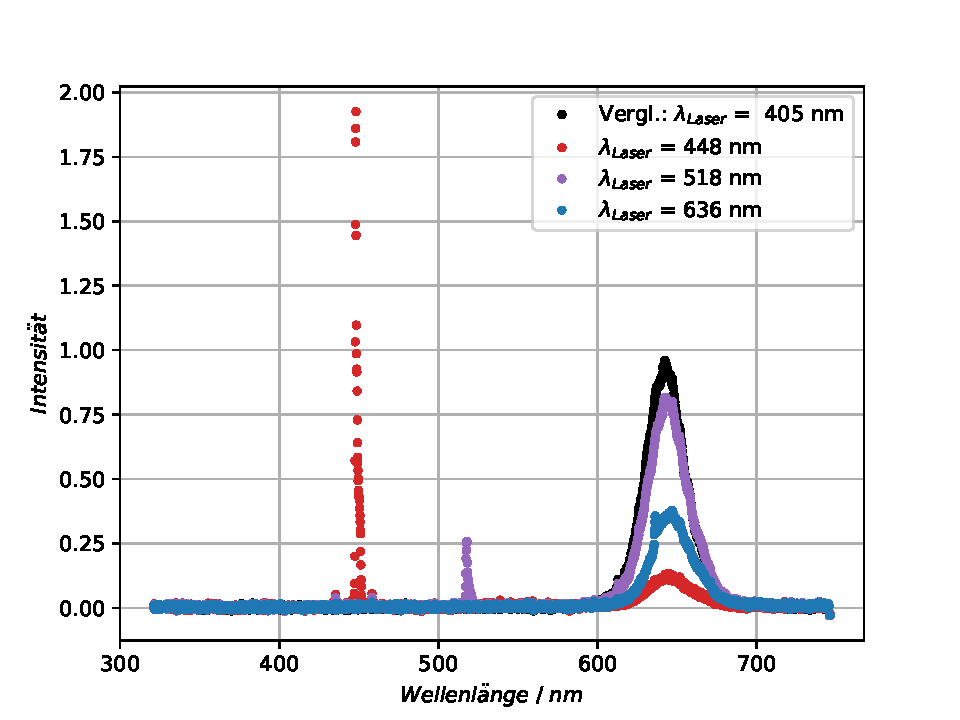
\includegraphics[width=\textwidth]{Plots/aufgabe2P1.pdf}
	\caption{PL-Spektren der Probe 1 mit unterschiedlicher Anregungswellenl\"{a}nge.}
	\label{abb:auf2p1a}
	\end{subfigure}
	~
	\begin{subfigure}[t]{0.45\textwidth}
	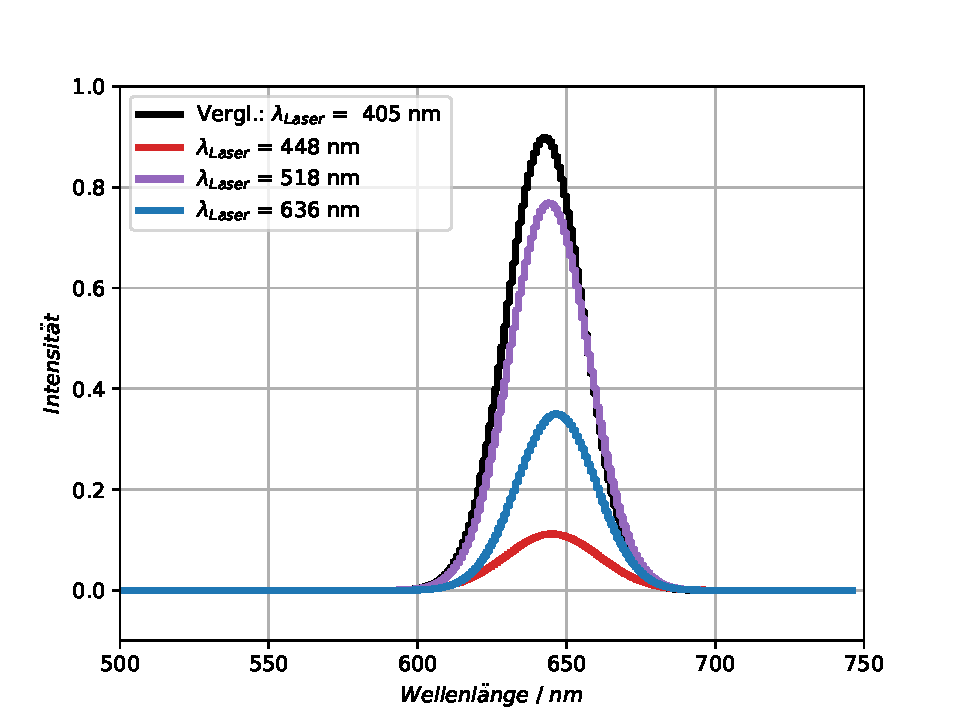
\includegraphics[width=\textwidth]{Plots/aufgabe2P1_fit_1s.pdf}
	\caption{Darstellung der Fits der PL-Peaks.}
	\label{abb:auf2p1b}
	\end{subfigure}
\caption{Messungen und Ergebnisse zur Probe 1.}
\label{abb:auf2P1}
\end{figure}
Die Messwerte, die aus den Fits abgelesen werden, sind in Tabelle (\ref{tab:auf2a}) notiert.
Hierbei steht die Abk\"{u}rzung Ref. f\"{u}r Reflexion und Emission wird mit Emi. bezeichnet.
Da sich der Reflexionspeak bei der Anregungswellenl\"{a}nge von $636 \, \text{nm}$ mit dem PL-Peak der Emission \"{u}berschneidet, konnte der Reflexionspeak hier nicht gefittet werden.
\begin{table}
	\centering
	\caption{Messergebnisse der Probe 1 zu Abbildung (\ref{abb:auf2P1})}
\begin{tabular}{|cccc|}
	\hline
	{$\lambda_{\text{Ref.}}$ / nm}	&	{Linienbreite Ref.}	&	{$\lambda_{\text{Emi.}}$ / nm}	&	{Linienbreite Emi.}	\\
	\hline
	448,32 & 0,69 & 645,31 & 18,47 \\
	517,99 & 0,85 & 644,23 & 15,73 \\
	- & - & 646,68 & 15,67 \\
	\hline
	\end{tabular}
\label{tab:auf2a}
\end{table}

Im Vergleich zu Probe 1 sind die PL-Peaks der Probe 2 (siehe Abbildung (\ref{abb:auf2p2b})) etwas schmaler.
Hier ist nun auff\"{a}llig, dass f\"{u}r eine Anregung mit $636 \, \text{nm}$ keine Photolumineszenz auszumachen ist.
\begin{figure}[hbtp]
\centering
	\begin{subfigure}[t]{0.45\textwidth}
	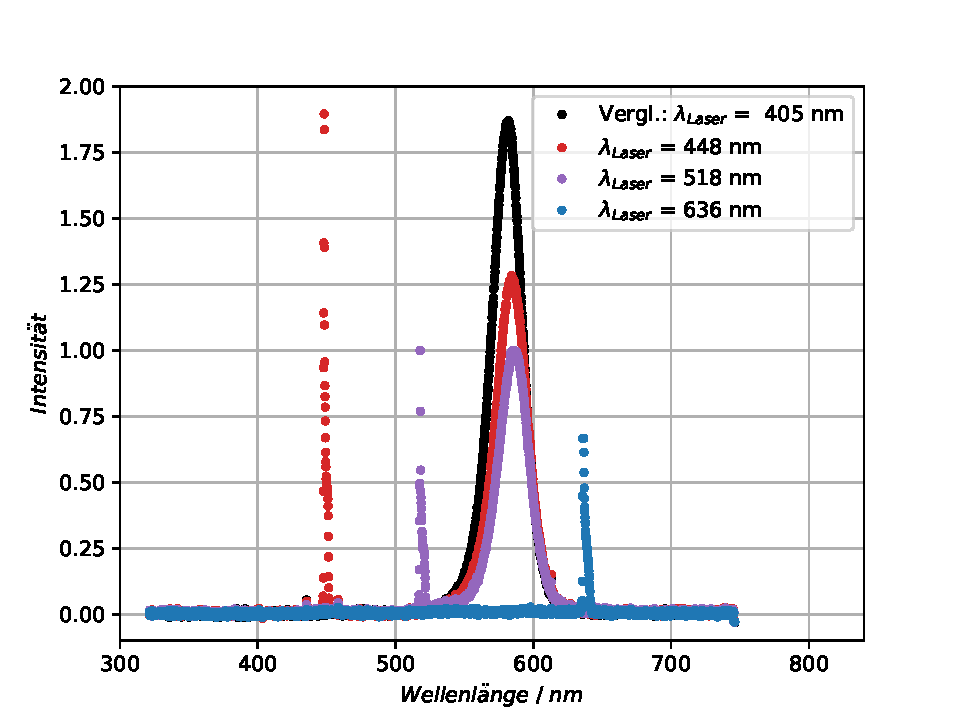
\includegraphics[width=\textwidth]{Plots/aufgabe2P2.pdf}
	\caption{PL-Spektren der Probe 2 mit unterschiedlicher Anregungswellenl\"{a}nge.}
	\label{abb:auf2p2a}
	\end{subfigure}
	~
	\begin{subfigure}[t]{0.45\textwidth}
	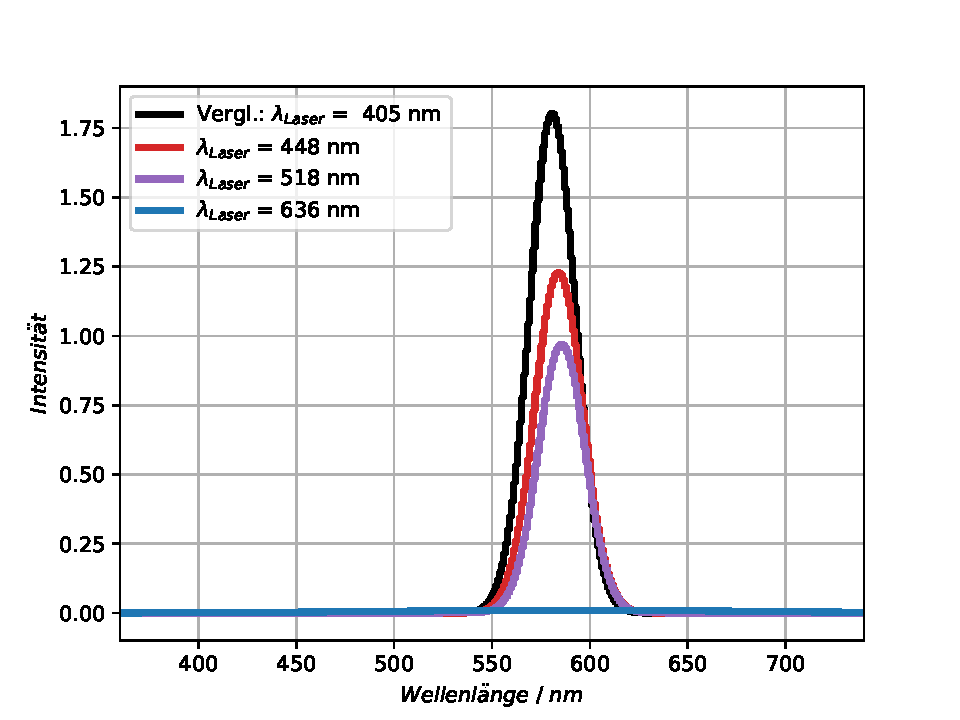
\includegraphics[width=\textwidth]{Plots/aufgabe2P2_fit_1s.pdf}
	\caption{Darstellung der Fits der PL-Peaks.}
	\label{abb:auf2p2b}
	\end{subfigure}
\caption{Messungen und Ergebnisse zur Probe 2.}
\label{abb:auf2P2}
\end{figure}
Werden die dazugeh\"{o}rigen Parameter aus Tabelle (\ref{tab:auf2b}) hinzugezogen ist festzustellen, dass die Linienreite eine ganze Gr\"{o}{\ss}enordungen gr\"{o}{\ss}er ist, als die der anderen PL-Peaks.
Die Messung k\"{o}nnte daher vernachl\"{a}ssigt werden, wird hier jedoch der Vollst\"{a}ndigkeit halber mit angegeben.
\begin{table}
	\centering
	\caption{Messergebnisse der Probe 2 zu Abbildung (\ref{abb:auf2P2})}
\begin{tabular}{|cccc|}
	\hline
	{$\lambda_{\text{Ref.}}$ / nm}	&	{Linienbreite Ref.}	&	{$\lambda_{\text{Emi.}}$ / nm}	&	{Linienbreite Emi.}	\\
	\hline
	448,50 & 0,93 & 584,02 & 14,44 \\
	518,19 & 1,05 & 585,65 & 14,09 \\
	636,97 & 1,62 & 589,88 & 109,10 \\
	\hline
	\end{tabular}
\label{tab:auf2b}
\end{table}

Zu letzt wird die Probe 3 mit unterschiedlichen Wellenl\"{a}ngen angeregt.
Wie schon bei der vorherigen Probe zu sehen, ist auch hier f\"{u}r eine Anregung mit $636 \, \text{nm}$ keine Photolumineszenz auszumachen.
\begin{figure}[hbtp]
\centering
	\begin{subfigure}[t]{0.45\textwidth}
	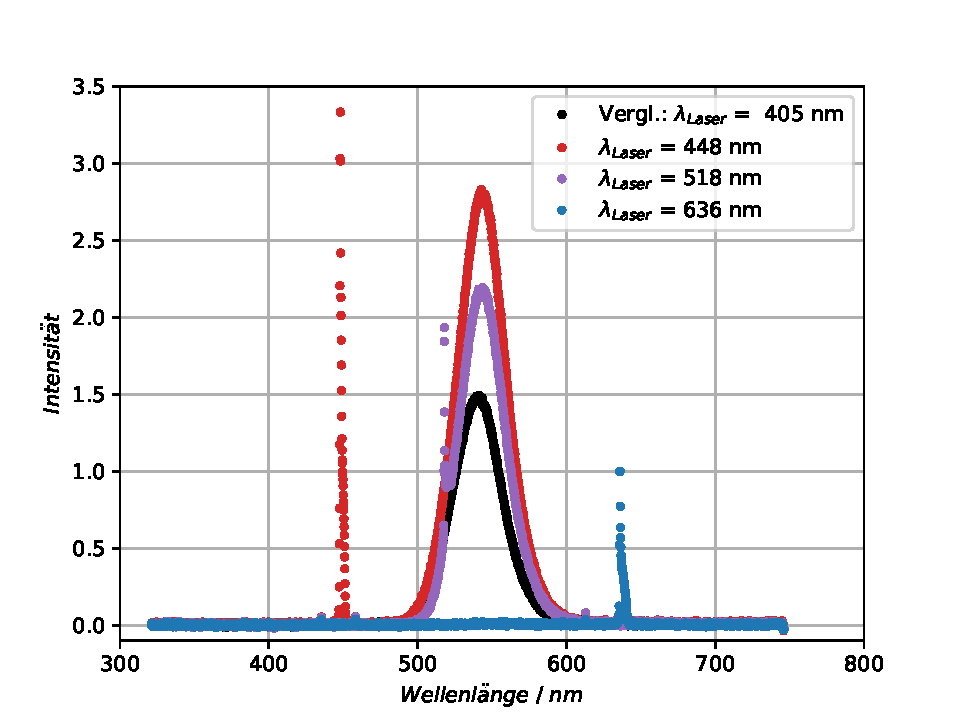
\includegraphics[width=\textwidth]{Plots/aufgabe2P3.pdf}
	\caption{PL-Spektren der Probe 3 mit unterschiedlicher Anregungswellenl\"{a}nge.}
	\label{abb:auf2p3a}
	\end{subfigure}
	~
	\begin{subfigure}[t]{0.45\textwidth}
	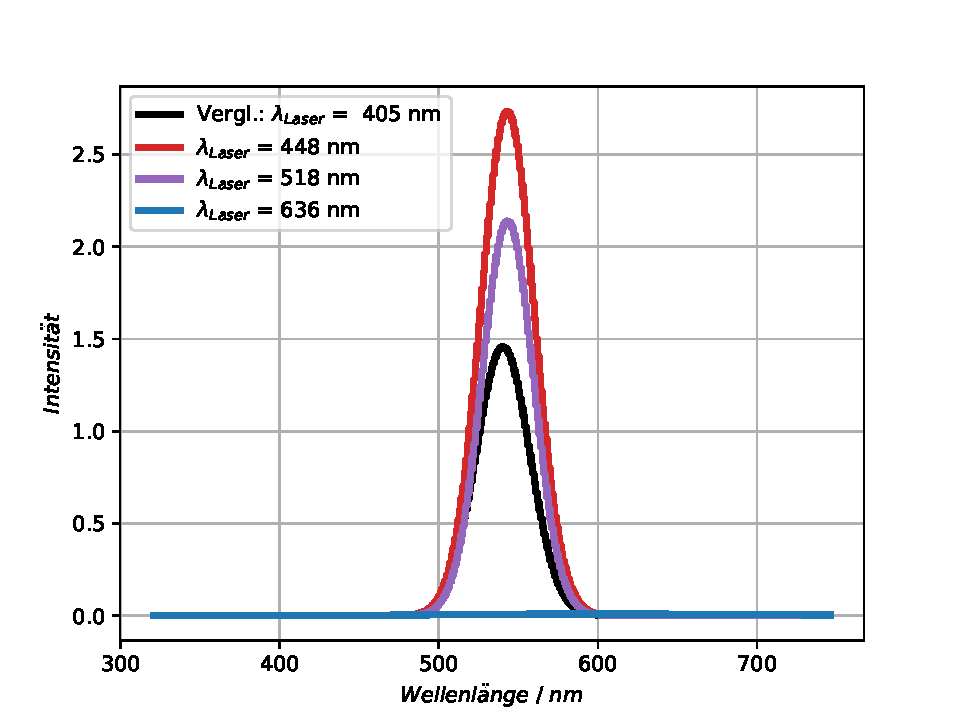
\includegraphics[width=\textwidth]{Plots/aufgabe2P3_fit_1s.pdf}
	\caption{Darstellung der Fits der PL-Peaks.}
	\label{abb:auf2p3b}
	\end{subfigure}
\caption{Messungen und Ergebnisse zur Probe 3.}
\label{abb:auf2P3}
\end{figure}
Auch hier ist die Linienbreite wieder eine ganze Gr\"{o}{\ss}enordungen gr\"{o}{\ss}er, als die der anderen PL-Peaks (siehe Abildung (\ref{tab:auf2c})).
\begin{table}
	\centering
	\caption{Messergebnisse der Probe 3 zu Abbildung (\ref{abb:auf2P3})}
\begin{tabular}{|cccc|}
	\hline
	{$\lambda_{\text{Ref.}}$ / nm}	&	{Linienbreite Ref.}	&	{$\lambda_{\text{Emi.}}$ / nm}	&	{Linienbreite Emi.}	\\
	\hline
	448,36 & 0,82 & 543,13 & 19,79 \\
	517,96 & 0,20 & 543,34 & 19,05 \\
	636,58 & 1,42 & 610,95 & 100,88 \\
	\hline
	\end{tabular}
\label{tab:auf2c}
\end{table}

Bei einem Vergleich aller drei Proben ist festzustellen, das die PL-Peaks nur sehr wenig gegeneinander auf der x-Achse verschoben sind und lediglich die Intensit\"{a}ten stakt unterschiedlich sind.

\subsection{Linearer Polarisationsgrad von Flüssigkeiten (Bonus-Aufgabe)}
Zu letzt wird der Polarisationsgrad einer Wein-Probe bestimmt.
Mit einem Laser der Wellenl\"{a}nge von $405 \, $nm wird diese angeregt.
Sowohl im Anregungspfad also auch im Detektionspfad wird die Polarisation mittels eines Filters varriert.
Es werden vier Spektren mit unterschiedlicher Polarisation aufgenommen, diese sind in Abbildung (\ref{abb:auf3}) zu sehen.
\begin{figure}[hbtp]
\centering
	\begin{subfigure}[t]{0.45\textwidth}
	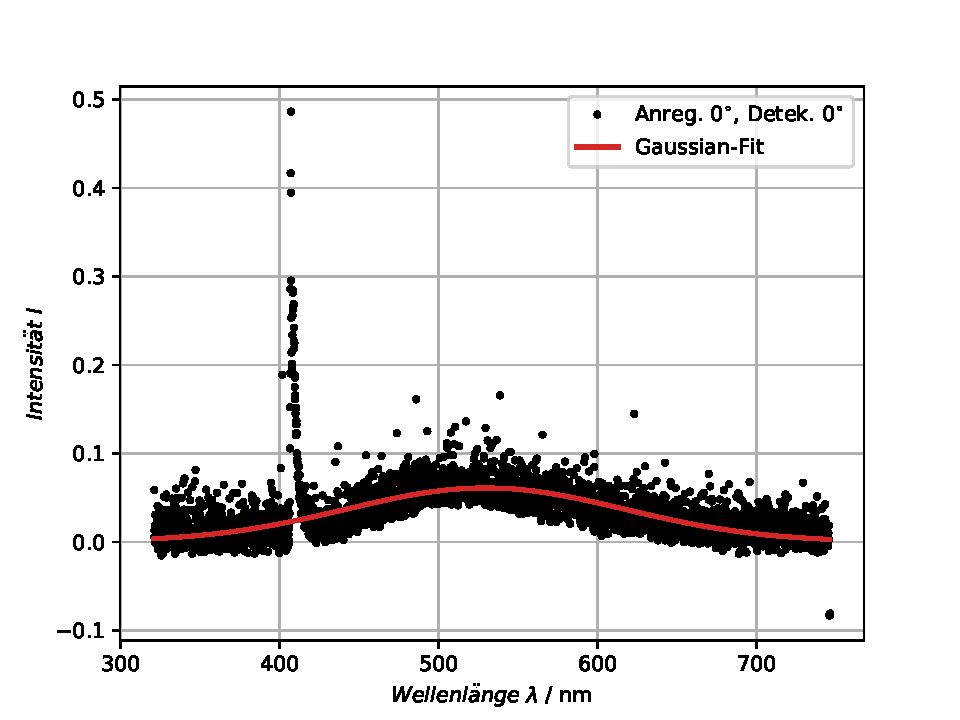
\includegraphics[width=\textwidth]{Plots/aufgabe3_P1.pdf}
	%\caption{}
	%\label{}
	\end{subfigure}
	%~
	\begin{subfigure}[t]{0.45\textwidth}
	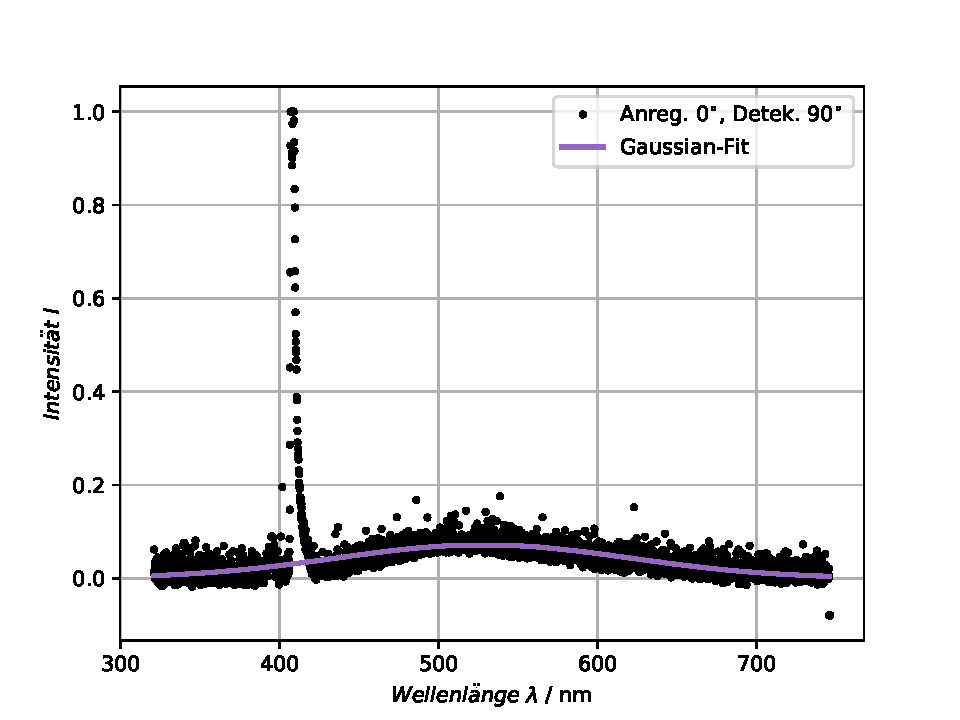
\includegraphics[width=\textwidth]{Plots/aufgabe3_P2.pdf}
	%\caption{.}
	%\label{}
	\end{subfigure}
	\\
	\begin{subfigure}[t]{0.45\textwidth}
	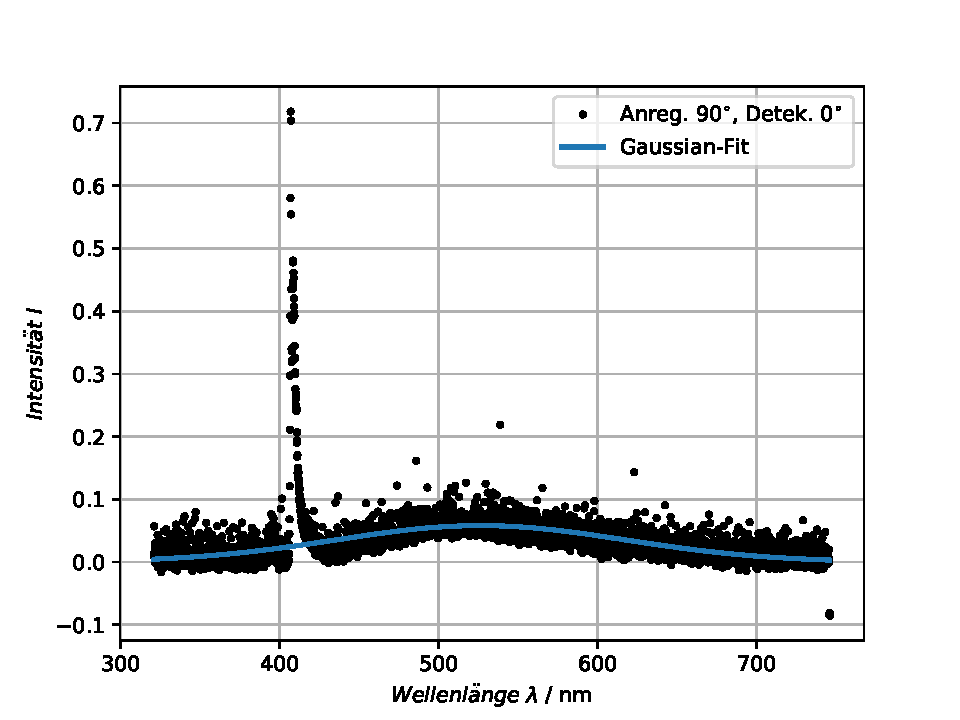
\includegraphics[width=\textwidth]{Plots/aufgabe3_P3.pdf}
	%\caption{}
	%\label{}
	\end{subfigure}
	%~
	\begin{subfigure}[t]{0.45\textwidth}
	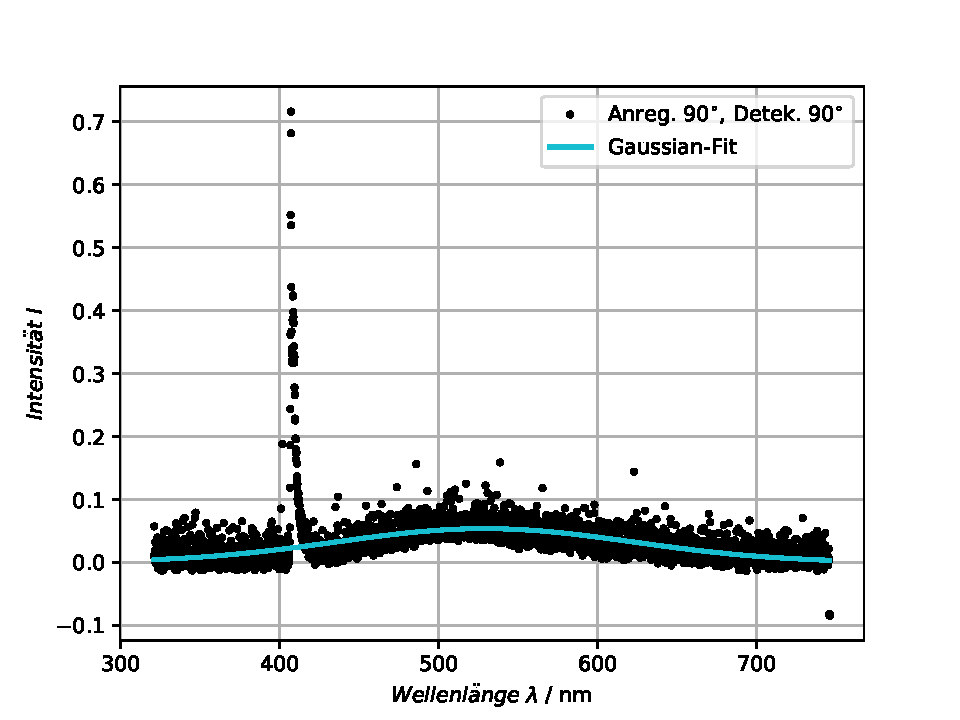
\includegraphics[width=\textwidth]{Plots/aufgabe3_P4.pdf}
	%\caption{.}
	%\label{}
	\end{subfigure}
\caption{Die PL-Spektren der Messungen von der Wein-Probe f\"{u}r verschiedene Polarisationspfade.}
\label{abb:auf3}
\end{figure}
Wie auch schon im vorherigen Aufgabenteil werden die sehr schalen Peaks in den Spektren durch eine Reflektion des Lasers hervorgerufen.
Die PL-Peaks werden mit Formel (\ref{form:gauss}) gefittet.
F\"{u}r einen besseren Vergleich der vier Messungen miteinander sind die Fit-Kurven in Abbildung (\ref{abb:auf3_vergleich}) dargestellt.
\begin{figure}[hbtp]
\centering
	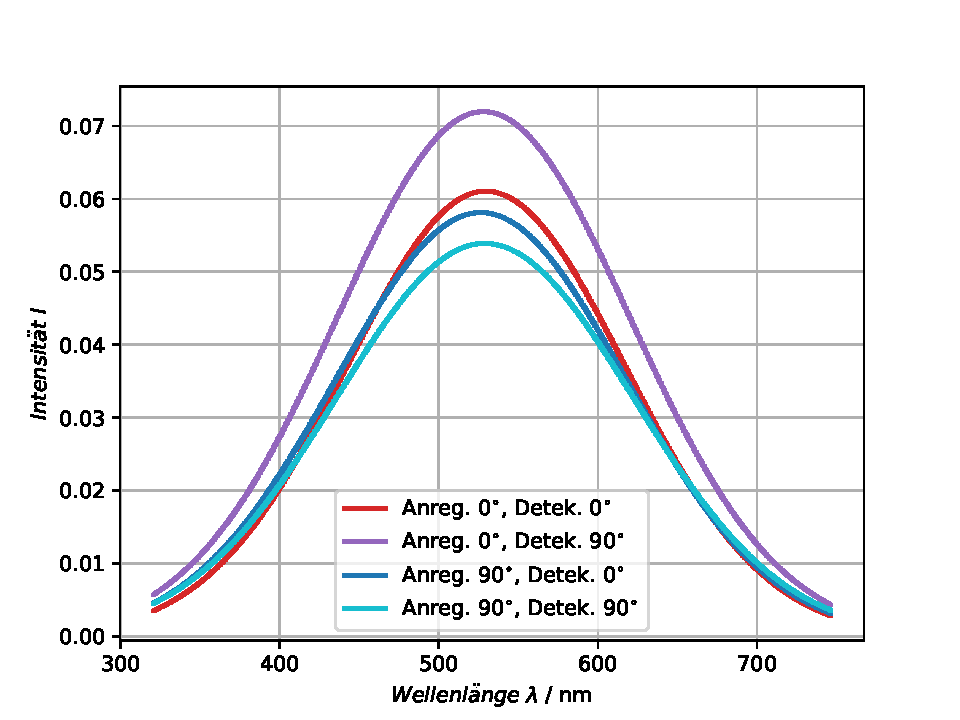
\includegraphics[width=0.6\textwidth]{Plots/aufgabe3_vergleich.pdf}
	\caption{Die gefitteten Gau{\ss}-Kurven der vier gemessenen PL-Spektren im Vergleich.}
	\label{abb:auf3_vergleich}
\end{figure}
Die Position $x_0$ des Maximuns der Gau{\ss}-Kurven ist untereinander ein wenig verschoben.
Auff\"{a}lliger sind die unterschiedlichen Intensit\"{a}ten der Maxima, welche in der danebenstehenden Tabelle (\ref{tab:auf3_vergleich}) notiert sind.
\begin{table}
\centering
\caption{Messwerte zu den gefitteten Gau{\ss}-Kurven.}
	\begin{tabular}{|rrcc|}
	\hline
	{Anregung} & {Detektion} & {Intensit\"{a}tsmaximum} & {Wellen\"{a}nge $\lambda$ / nm}\\
	\hline
	$0^{\circ}$ & $0^{\circ}$ & 0,0611 & 529,767 \\
	$0^{\circ}$ & $90^{\circ}$ & 0,0719 & 528,218\\
	$90^{\circ}$ & $0^{\circ}$ & 0,0581 & 526,574\\
	$90^{\circ}$ & $90^{\circ}$ & 0,0539 & 529,072\\
	\hline
\end{tabular}
\label{tab:auf3_vergleich}
\end{table}
Aus den Intensit\"{a}tsmaxima wird mittels der Formel (\ref{form:polar}) der Polarisationsgrad berechnet.
\begin{equation}
	\text{Polarisationsgrad} = \frac{I_{PL,0^{\circ}} - I_{PL,90^{\circ}}}{I_{PL,0^{\circ}} + I_{PL,90^{\circ}}}
	\label{form:polar}
\end{equation}
F\"{u}r $0^{\circ}$ beziehungsweise $90^{\circ}$ im Anregungspfad ergeben sich damit die folgenden Werte des Polarisationsgrad.
\begin{align*}
	\text{P}_{0^{\circ}} &= 0,08204 \\
	\text{P}_{90^{\circ}} &= 0,03779 \\	
\end{align*}
